% !TEX TS-program = lualatex-dev
\DocumentMetadata{lang=en,tagging=on,
  pdfstandard=ua-2,tagging-setup={math/setup=mathml-SE,math/alt/use}
}%,uncompress
\AtBeginDocument{\tagpdfsetup{role/new-tag=frametitle/H1}}
\documentclass{ltx-talk}
\usepackage{multirow}
\usepackage{tikz}
\usepackage{booktabs}
\usepackage{qrcode}
\usepackage{unicode-math}
\usepackage{bookmark}
\usepackage{emoji}
\usepackage{table-header-scope}

\title{\texorpdfstring{\LaTeX}{LaTeX} PDF accessibility}
\author{Tim Prescott}
\institute[UND]{University of North Dakota}
%\date{August 27, 2025}
% UND abstract:
% We'll discuss how to use LaTeX to create accessible pdfs (including presentations), how to check how well you've accomplished that task, and our successes and failures thus far.
\date{October 11, 2025}
% MAA abstract:
% The US DoJ has announced an April deadline to comply with federal requirements to provide accessible course materials.  Over the past few years, LaTeX has rapidly improved the accessibility of its pdfs.  We'll discuss how to create accessible pdfs (including presentations), how to check how well you've accomplished that task, and our successes and failures thus far.
% 15-20 min

%\providecolor{maybeUNDgreen}{Hsb}{146,1,0.62}
\providecolor{maybeUNDgreen}{Hsb}{146,1,0.53}

\EditInstance{header}{std}{
  background-color = maybeUNDgreen,
  color            = white,
}

\EditInstance{footer}{std}{
  color         = black!75,
  separator     = \hfill|\hfill,
  element-order = {date, author, title, institute, framenumber},
  right-skip    = 3mm,
  left-skip     = 3mm,
}

% qrcode modification from https://tex.stackexchange.com/a/718275/107497
\makeatletter
\ExplSyntaxOn
\cs_new_protected:Npn\qr@savepos 
 {
  \tex_savepos:D 
  \RecordProperties{qr@save-\theqrcodecnt}{xpos,ypos}
  \tex_savepos:D 
 }
\cs_new:Npn \qr@diminbp #1 {\dim_to_decimal_in_bp:n {#1}}
\ExplSyntaxOff

\newcounter{qrcodecnt}
\NewSocket{tagsupport/qrcode/begin}{0}
\NewSocket{tagsupport/qrcode/end}{0}
\NewSocketPlug{tagsupport/qrcode/begin}{tag}
 {%
   \leavevmode
   \tagmcend%
   \stepcounter{qrcodecnt}\qr@savepos%
   \ExpandArgs{e}\tagpdfsetup
     {role/new-attribute=
      {qrcode-\theqrcodecnt}
      {
       /O /Layout 
       /BBox [\qr@diminbp{\RefProperty{qr@save-\theqrcodecnt}{xpos}sp}
              \qr@diminbp{\RefProperty{qr@save-\theqrcodecnt}{ypos}sp-0.5\qr@desiredheight}
              \qr@diminbp{\RefProperty{qr@save-\theqrcodecnt}{xpos}sp+\qr@desiredheight} 
              \qr@diminbp{\RefProperty{qr@save-\theqrcodecnt}{ypos}sp+0.5\qr@desiredheight}] 
      }%
     }%
   \tagstructbegin{tag=Figure,alt=\qr@texttoencode,
    attribute=qrcode-\theqrcodecnt}%
   \tagmcbegin{}%
  }
  
\NewSocketPlug{tagsupport/qrcode/end}{tag} 
 {\tagmcend\tagstructend\tagmcbegin{}}
 
\AssignSocketPlug{tagsupport/qrcode/begin}{tag} 
\AssignSocketPlug{tagsupport/qrcode/end}{tag} 

\def\qrcode@hyperwrapper@hyperref#1{%
  \href{\qr@texttoencode}%
   {\UseTaggingSocket{qrcode/begin}\SuspendTagging{qrcode}%
    #1\ResumeTagging{qrcode}\UseTaggingSocket{qrcode/end}}}
 
\def\qrcode@hyperwrapper@nohyperref#1{%
  \UseTaggingSocket{qrcode/begin}\SuspendTagging{qrcode}%
  #1\ResumeTagging{qrcode}\UseTaggingSocket{qrcode/end}}

\patchcmd\qrcode@int{\relax}{\qrcode@hyperwrapper@nohyperref}{}{\fail}

\makeatother


\begin{document}

\section{\texorpdfstring{\LaTeX}{LaTeX} PDF accessibility}

\begin{frame}
\maketitle
\end{frame}

\begin{frame}
\frametitle{Preamble}
\framesubtitle{Everything will be online}
The pdf of this talk and other resources will be posted online, so you don't need to write down what you see here.
\end{frame}

%\begin{frame}
%\tableofcontents
%\end{frame}

\begin{frame*}
\frametitle{TL;DR}
Update \LaTeX, use
\begin{verbatim}
\DocumentMetadata{lang=en,tagging=on,pdfstandard=ua-2,
  tagging-setup={math/setup=mathml-SE,math/alt/use}}
\documentclass{article}
...
\usepackage{unicode-math}
\title{...}
\end{verbatim}
compile with Lua\LaTeX, and maybe it all works just fine.\\
\texttt{math/alt/use} $\Leftrightarrow$ Blackboard Ally\\\bigskip
Optional warmups: \verb|\RequirePackage{nag}| or\\
\qquad\texttt{pdfstandard=ua-1,pdfversion=1.7} (but not \texttt{math/setup=mathml-SE})
\end{frame*}

\section{How to \TeX\ an accessible PDF}

\begin{frame}
\frametitle{Basic idea}
Use \LaTeX\ so that the output looks how you want it\\
\textbf{and the input reflects the meaning.}\\
(Don't use tabular to position boxes.)
\end{frame}

\begin{frame}
\frametitle{After the basics --- Tables}
\begin{itemize}
\item\texttt{\textbackslash tagpdfsetup\{table/header-rows=\{...\},table/header-columns=\{...\}\}\\
\qquad\qquad \textrm{outside of the} tabular\\
\qquad\qquad \textrm{(lasts until the group} \textbackslash ends)}
\item\texttt{\textbackslash tagpdfsetup\{table/multirow=\{\emph{number of rows}\}\}} 
\item Interface will probably change
%\item Need to work around a PAC bug
%\item And PAC still doesn't like multi(row/column) in the data
\end{itemize}
\end{frame}

\begin{frame}
\frametitle{After the basics --- Images}
\begin{itemize}
\ttfamily
\item\textbackslash includegraphics[\textbf{alt=\{...\}}]
\item\textbackslash tikz[\textbf{alt=\{...\}}]
\item\textbackslash begin\{tikzpicture\}[\textbf{alt=\{...\}}]
\item\textbackslash begin\{picture\}[\textbf{alt=\{...\}}]
\end{itemize}
Keep it brief and objective; exposition won't be seen by most students.\\
Alternatives to {\bfseries\ttfamily alt=\{...\}} are {\bfseries\ttfamily artifact} and {\bfseries\ttfamily actualtext=\{...\}}.
%\\
%PAC objects to a bug in pgfplots.
\end{frame}

% cut for MAA
%\begin{frame}
%\frametitle{TTaDA: Making Simple Images Accessible}
%\begin{itemize}
%\item At most 120 characters or 1--2 sentences
%\item Usually not seen
%\item Specific, accurate, objective, neutral
%\item What does my audience need from this picture?
%\item Do not begin with ``image''
%\item Do not repeat the caption
%\item Artifact/decorative $\Leftrightarrow$ unnecessary
%\end{itemize}
%\end{frame}
%%
%\begin{frame}
%\frametitle{TTaDA: Making Complex Images Accessible}
%If alt text would require more than 120 characters or 1--2 sentences:
%\begin{itemize}
%\item Write it up separately
%\item Alt text sentence 1: what it is
%\item Alt text sentence 2: where to find the separate description
%\end{itemize}
%\end{frame}

\begin{frame}
\frametitle{Tools}
To verify that a pdf is accessible:
\begin{description}
\item[Ally, Siteimprove:] (Commercial addons)
\begin{itemize}
\item[\emoji{thumbsup}] easy to pass, checks color contrast
\item[\emoji{thumbsdown}] too easy, false negatives
\end{itemize}
\item[VeraPDF:] \url{https://verapdf.org/software}
\begin{itemize}
\item[\emoji{thumbsup}] has command line option; \LaTeX\ team
\item[\emoji{thumbsdown}] no GUI for pdf errors
\end{itemize}
\item[PDFix:] \url{https://pdfix.net}
\begin{itemize}
\item[\emoji{thumbsup}] GUI
\item[\emoji{thumbsdown}] no command line
\end{itemize}
\item[PAC:] \url{https://pac.pdf-accessibility.org/en}
\begin{itemize}
\item[\emoji{thumbsdown}] Windows only; maxes out at UA-1/1.7; bug with tabular headers
\item[\emoji{thumbsup}\emoji{thumbsdown}] more thorough (pgfplots, multi[row|column])
\end{itemize}
\end{description}
\end{frame}

% cut for MAA
%\section{Tools}
%%
%\begin{frame}
%\frametitle{PDFix --- \url{https://pdfix.net}}
%\centering
%
\includegraphics[alt={Screenshot of PDFix},height=\textheight]{pdfixScreenshot}
%\end{frame}
%%
%\begin{frame}
%\frametitle{VeraPDF --- \url{https://verapdf.org/software}}
%\centering
%
\includegraphics[alt={Screenshot of VeraPDF},height=\textheight]{veraPdfScreenshot}
%\end{frame}
%%
%\begin{frame}
%\frametitle{PAC --- \url{https://pac.pdf-accessibility.org/en}}
%\centering
%
\includegraphics[alt={Screenshot of PAC},height=\textheight]{PacScreenshot}
%\qquad
%\raisebox{.5\textheight}{\parbox{.5\linewidth}{A bit more streamlined, but:
%\begin{itemize}
%\item Windows only
%\item maxes out at UA-1/1.7
%\item objects to bug in pgfplots
%\item has a bug with tables
%\item doesn't like multi(row/column)
%\end{itemize}}}
%\end{frame}

\section{Specific packages \& classes}

\begin{frame}
\frametitle{Replacements \& Adjustments}
\begin{itemize}
\item enumitem \& enumerate \textrightarrow\ enumext or nothing (new syntax)
\item margin[fit|fix|note] \textrightarrow\ margin[alia|par]
\item Beamer \textrightarrow\ ltx-talk (lualatex-dev, mostly same syntax)
\item Some packages need some (or a lot of) help (tcolorbox, titlesec, qrcode, media9, \ldots)
\end{itemize}
\end{frame}

\begin{frame*}
\frametitle{ltx-talk}\pause
\begin{itemize}[<+->]
\item Same \verb|\pause|/overlay specification idea (eg, \verb|\begin{itemize}[<+->]|)
\item ``\emph{highly} experimental'' --- must use \texttt{lualatex-dev} (for another month?)
\item Ally $\Rightarrow$ \verb|\AtBeginDocument{\tagpdfsetup{role/new-tag=frametitle/H1}}|
\item Can ``easily'' specify header and footer information\\\bigskip
\hfill%
\alt<+->{%
 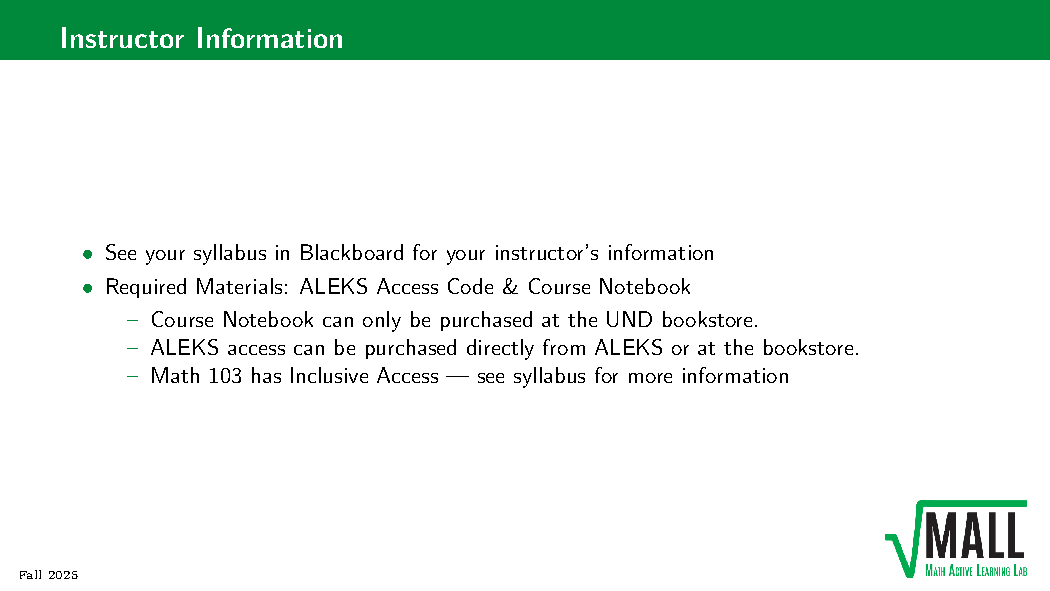
\includegraphics[height=.4\textheight,alt={MALL presentation with logo in corner}]{Blackboard-PPT-Tues.pdf}%
}{%
 \parbox[c][.4\textheight]{1em}{}%
}%
\hfill\null
\end{itemize}
\end{frame*}

% cut for MAA
%\begin{frame}
%\frametitle{Colors}
%\begin{itemize}
%\item UND green is $\operatorname{RGB}(0,158,68)=\operatorname{Hsb}(146,1,0.62)$
%\item UND orange is $\operatorname{RGB}(255,103,31)=\operatorname{Hsb}(19,0.88,1)$
%\item Insufficient contrast with white?
%\item Add 13\% and 22\% black.
%\item Also red with white (hyperref)
%\end{itemize}
%\end{frame}

% debugging ?

\begin{frame*}
\frametitle{For more information}
\begin{itemize}
\item \url{https://latex3.github.io/tagging-project/documentation/prototype-usage-instructions.html}
\item \url{https://latex3.github.io/tagging-project/tagging-status/}
\item \texttt{texdoc: documentmetadata-support-code, latex-lab-table, enumext, ltx-talk}
\item \url{https://www.texdev.net/ltx-talk/examples/}
\item Compiling needs more time (x7), RAM (x4), strings\&hash entries (x11), larger pdf (x2.5)\\
\qquad try \verb|\DocumentMetadata{lang=en}| for draft runs
\item \url{https://www.youtube.com/watch?v=Eu_qM53tInw&t=5900s}\\
\qquad A before and after example using Foxit, NVDA, and MathCAT
\end{itemize}
\end{frame*}

\section{Current status}

\begin{frame}
\newcommand{\mynote}[1]{\makebox[0pt][l]{\textsuperscript{#1}}}
\frametitle{Current status}
\vfill
\centering\tagpdfsetup{table/header-rows={1}}
\begin{tabular}{ @{} lcccccc @{} }
\tagpdfsetup{table/multirow={2}}\multirow{2}{*}{Document} & BB & UND.edu & PAC & \multicolumn{2}{c}{VeraPDF} & \tagpdfsetup{table/multirow={2}}\multirow{2}{*}{\LaTeX ML}\\
& Ally & SiteImprove & UA-1 & UA-1 & UA-2 & \\\midrule
%Math Track Meet Dec 2023 & 100\% & Y & Y & Y & Y & Y \\ % cut for MAA
%Math Track Meet 2025 & 100\% & Y & Y & Y & Y & Y \\ % cut for MAA
Calculus (Apex UND) & 100\% & Y & N & Y\mynote{***} & Y\mynote{***} & ``Y'' \\
Linear Algebra (Cherney UND) & 100\% & ``Y'' & Y\mynote* & Y\mynote* & Y\mynote* & Y\mynote* \\
this talk & 100\%\mynote* & ``Y'' & Y\mynote* & Y\mynote* & Y\mynote* & N \\
%MALL syllabus${}\times37$ & 100\% & ``Y'' & Y\mynote* & Y\mynote* & Y\mynote* & Y\mynote* \\\addlinespace % cut for MAA
%Simple Syllabus & 5\% & ``N'' & N & N & N & N/A %\\ % cut for MAA
%\bottomrule
\end{tabular}
\vfill

\hspace{.2\textwidth}
\begin{minipage}{.6\textwidth}
\raggedright
\footnotesize
``Presumed'', \textsuperscript*With help\\
Calculus: PAC: Multi(row/column), pgfplots
\end{minipage}
\vfill
\end{frame}

\begin{frame}
\frametitle{Examples}\tagpdfsetup{table/header-rows={1}}
\begin{tabular}{l p{.2\textwidth} p{.5\textwidth}}
Math & before & after \\\midrule
$a^2+b^2=c^2$ & ay two plus bee two equals cee two & ay squared plus bee squared is equal to cee squared\\\addlinespace[4ex]
{$\begin{pmatrix}a&b\\c&d\end{pmatrix}^{-1}$} & minus one list with one item ay bee cee dee & two lines line one ay bee line two cee dee to the negative one power \\\addlinespace[4ex]
{$\begin{pmatrix}1&2\\3&4\end{pmatrix}\begin{pmatrix}1&1\\0&1\end{pmatrix}$} & three four one two zero one one one & the two by two matrix row one one two row two three four times the two by two matrix row one one one row two zero one
\end{tabular}
\end{frame}

\begin{frame}
\frametitle{Promised Resources}\centering
\vfill
\url{https://sites.und.edu/timothy.prescott/accessible}\\\vfill
\qrcode[height=.6\textheight]{https://sites.und.edu/timothy.prescott/accessible}\vfill
\end{frame}

\end{document}
